
\section{Υποσύστημα κίνησης}


%
% Κινητήρες
%

\subsection{Παραγωγή σήματος\slash κίνησης}

Σύμφωνα με εγχειρίδιο χρήσης της \textcite{hitec02}, όλοι οι κινητήρες της
λειτουργούν σε τάση 4.8--6V δεχόμενοι τετραγωνικό σήμα ελέγχου με διαμόρφωση
PWM (\textenglish{Pulse-Width Modulation}) 3--5V σε συχνότητα ανανέωσης 50Hz.
Η διάρκεια των παλμών κυμαίνεται μεταξύ 0.9ms και 2.1ms, με παλμούς των 1.5ms να
χρησιμοποιούνται για την ακινητοποίησή τους \parencite{hitec02}.

Οι παραγωγή των παλμών μπορεί να πραγματοποιηθεί είτε με λογισμικό είτε από
κάποιο διαθέσιμο κύκλωμα Χρονομετρητή\slash Απαριθμητή (\textenglish{Timer\slash
Counter}) του μικροελεγκτή. Το κύριο πλεονέκτημα του λογισμικού είναι η
ελευθερία επιλογής οποιουδήποτε ακροδέκτη για την έξοδο του σήματος καθώς και η
δυνατότητα παραγωγής πολλαπλών τέτοιων σημάτων που περιορίζονται από το συνολικό
πλήθος ακροδεκτών ή τη συχνότητα του ρολογιού συστήματος (όποιο είναι
μικρότερο).

Αντιθέτως, στην περίπτωση χρήσης κυκλωμάτων, το παραγόμενο σήμα διοχετεύεται
στους συγκεκριμένους ακροδέκτες με τους οποίους είναι το καθένα εσωτερικά
συνδεδεμένο και, σαφώς, το μέγιστο πλήθος παράλληλων σημάτων περιορίζεται από το
συνολικό αριθμό τέτοιων κυκλωμάτων. Επίσης, κάθε Χρονομετρητής\slash Απαριθμητής
υπόκειται σε πρόσθετους περιορισμούς, όπως το εύρος τιμών που υποστηρίζει ο
καθένας (για παράδειγμα, ανάλυση 8- ή 16-bit).

Ωστόσο, στη χρήση κυκλώματος Χρονομετρητή\slash Απαριθμητή συγκαταλέγονται και
ορισμένα σημαντικά πλεονεκτήματα.
Καθότι το σήμα παράγεται από ξεχωριστό κύκλωμα, η CPU του μικροελεγκτή είναι
διαθέσιμη για την εκτέλεση οποιασδήποτε άλλης εργασίας (για παράδειγμα, κάποιας
ρουτίνας εξυπηρέτησης διακοπής) παράλληλα με την παραγωγή του σήματος, χωρίς να
απαιτείται πολύπλεξη εργασιών (ώστε να αποδίδονται κβάντα τόσο στη γεννήτρια
σήματος όσο και σε κάποια άλλη εργασία). Ένα δεύτερο, λιγότερο σημαντικό για την
προκειμένη υλοποίηση, πλεονέκτημα είναι η δυνατότητα επίτευξης υψηλότερων
συχνοτήτων με πολύ λιγότερο θόρυβο (\textenglish{jitter}) και μεγαλύτερη
ακρίβεια.

Τελικά, για την παραγωγή σήματος PWM των κινητήρων επιλέγεται η χρήση κυκλώματος
Χρονομετρητή\slash Απαριθμητή καθώς, επιπροσθέτως των ανωτέρω πλεονεκτημάτων,
παρουσιάζει υψηλότερο ενδιαφέρον, από εκπαιδευτικής πλευράς.

\subsubsection{Γεννήτρια PWM}

Ο μικροελεγκτής ATmega328P διαθέτει δύο κυκλώματα Χρονομετρητή\slash Απαριθμητή
με δυνατότητα παραγωγής σήματος PWM. Ο πρώτος (Timer\slash Counter0) είναι 8-bit
και ο δεύτερος (Timer\slash Counter1), 16-bit. Για την επιλογή κάποιου, κρίνεται
σκόπιμη η περαιτέρω ανάλυση της λειτουργίας της γεννήτριας PWM καθώς και των
απαιτήσεων για το σήμα ελέγχου των κινητήρων.

Όσον αφορά τη γεννήτρια PWM, ο Χρονομετρητής\slash Απαριθμητής διαθέτει έναν
καταχωρητή μετρητή, τον TCNTn, ο οποίος σταδιακά αυξάνεται. Επίσης, διαθέτει
δύο ακόμα καταχωρητές, τους OCRnA και OCRnB, οι οποίοι αντιστοιχίζονται με
ακροδέκτες του μικροελεγκτή, αναφερόμενοι ως OCnA και OCnB. Μόλις η τιμή του
TCNTn γίνει ίση με την τιμή που περιέχεται είτε στον OCRnA είτε στον OCRnB,
είναι δυνατή η αλλαγή της εξόδου του αντίστοιχου ακροδέκτη. Ο TCNTn συνεχίζει
την ανοδική του πορεία έως ότου φτάσει την τιμή TOP. Από το σημείο αυτό και
ανάλογα με τη λειτουργία που έχει επιλεγεί, ο TCNTn είτε επανέρχεται ακαριαία
στην τιμή 0 και αρχίζει εκ νέου τον επόμενο κύκλο, είτε φθίνει σταδιακά μέχρι το
0, πάντα εναλλάσσοντας την τιμή των OCnA και OCnB όποτε εξισώνεται με τους OCRnA
και OCRnB, αντιστοίχως \parencite[100--102,124--129]{atmel13}.
Γίνεται αντιληπτό ότι η συχνότητα με την οποία αυξάνεται ο TCNTn καθώς και η
τιμή TOP επηρεάζουν τη συχνότητα του παραγόμενου σήματος. Παράλληλα, η τιμή των
OCRnA και OCRnB επηρεάζουν τον κύκλο εργασίας του (\textenglish{duty cycle}),
δηλαδή το τμήμα της περιόδου κατά το οποίο το παραγόμενο σήμα βρίσκεται σε
λογικό 1.

Η παραγωγή PWM υποστηρίζεται από τρεις ρυθμίσεις λειτουργίας των
Χρονομετρητών\slash Απαριθμητών, τις \textenglish{Fast PWM mode, Phase Correct
PWM mode (PCPWM)} και \textenglish{Phase and Frequency Correct PWM mode
(PFCPWM)}, εκ των οποίων οι δύο τελευταίες ενδείκνυνται για τον έλεγχο κινητήρων
εν γένει, και αυτό επειδή το παραγόμενο σήμα ανταποκρίνεται πιο ομαλά στις
αλλαγές της τιμής TOP \parencite[126,128]{atmel13}. Οι PCPWM και PFCPWM, εφόσον
η τιμή TOP -- η τιμή μέχρι την οποία αυξάνει ο TCNTn πριν αρχίσει τη φθίνουσα
πορεία του -- διατηρείται σταθερή κατά τη διάρκεια λειτουργίας του μετρητή,
είναι πανομοιότυπες \parencite[127]{atmel13}. Στην περίπτωση της υλοποίησης, η
συχνότητα του παραγόμενου σήματος είναι σταθερή, όπως έχει αναφερθεί, στα 50Hz
και, συνεπώς, το ίδιο ισχύει για την τιμή TOP. Ως αποτέλεσμα, οι λειτουργίες
PCPWM και PFCPWM είναι ισοδύναμες για τις ανάγκες της υλοποίησης και μπορεί να
προτιμηθεί είτε η μία είτε η άλλη, στην περίπτωση που επιλεγεί ο
\textenglish{Timer\slash Counter1}, ή η PCPWM, στην περίπτωση που επιλεγεί ο
\textenglish{Timer\slash Counter0}, καθώς σύμφωνα με τις επιλογές παραγωγής
κυματομορφής της \textcite[107]{atmel13}, ο \textenglish{Timer\slash Counter0}
υποστηρίζει μόνο αυτήν.

Στις λειτουργίες PCPWM και PFCPWM, η συχνότητα του παραγόμενου σήματος παρέχεται
από τη σχέση \parencite[102,128,129]{atmel13}:
\begin{equation}
\label{eq:motor:f_pwm}
f_{PWM} = \frac{f_{clk_{I/O}}} {2\;N\;TOP}
\end{equation}

\noindent όπου, \\
\begin{tabu}{X[-1] @{ : }  X}
$f_{clk_{I/O}}$ & Συχνότητα ρολογιού που λαμβάνουν οι μετρητές (καθώς και
                  άλλα περιφερειακά, όπως SPI).                               \\
$N$             & Τιμή υποδιαίρεσης ρολογιού για χρήση από τους μετρητές (1,
                  8, 64, 256 ή 1024).                                         \\
$TOP$           & Η μέγιστη τιμή που παίρνει ο TCNTn.
\end{tabu}

Η συχνότητα ρολογιού, $f_{clk_{I/O}}$, της υλοποίησης ορίζεται στα 4MHz, ενώ
έχει ήδη αναφερθεί η επιθυμητή συχνότητα του παραγόμενου σήματος, $f_{PWM}$,
(50Hz). Η τιμή υποδιαίρεσης, $N$, προσδιορίζεται από τα bit CSn2:0 του
καταχωρητή TCCRnB, και επιτρέπει τη μείωση της συχνότητας των μετρητών. Η χρήση
της τιμής $TOP$ έχει αναφερθεί προηγουμένως. Η τιμή της προσδιορίζεται κατά την
επιλογή της λειτουργίας παραγωγής κυματομορφής μέσω των bit WGM των καταχωρητών
TCCRnA και TCCRnB. Στον πίνακα \ref{tab:motor:wgm} παρουσιάζονται ορισμένες
ρυθμίσεις PCPWM των δύο μετρητών. Σημειώνεται ότι στην περίπτωση του
\textenglish{Timer\slash Counter0}, οι δύο λειτουργίες που αναφέρονται είναι οι
μοναδικές PCPWM, ενώ στην περίπτωση του \textenglish{Timer\slash Counter1},
έχουν παραλειφθεί ορισμένες οι οποίες είναι παρόμοιες με την λειτουργία 1 του
\textenglish{Timer\slash Counter0} (δηλαδή, προκαθορισμένες σταθερές τιμές
0x00FF, 0x01FF και 0x3FF).

\begin{table}
    \caption{Μέρος ρυθμίσεων PCPWM των \textenglish{Timer\slash Counter0} και 1.
        \label{tab:motor:wgm}}

\begin{center}
\begin{tabu} spread 0pt
    {X[-1,C] X[-1,C] X[-1,C] X[-1,C] X[-1,C] X[-1,C] X[-1]}

    \rowfont\bfseries
                    & {Mode} & {WGMn3} & {WGMn2} & {WGMn1} & {WGMn0} & {TOP}  \\
    \tabucline{2-}
    Timer\slash
    Counter0        &      1 &      -- &       0 &       0 &       1 &  0xFF  \\
                    &      5 &      -- &       1 &       0 &       1 & OCR0A  \\
    Timer\slash
    Counter1        &     10 &       1 &       0 &       1 &       0 &  ICR1  \\
                    &     11 &       1 &       0 &       1 &       1 & OCR1A  \\
\end{tabu}

\floatfoot{Απόσπασμα \fullcite[107,133]{atmel13}}
\end{center}\end{table}

Οι λειτουργίες που παρέχουν μία προκαθορισμένη σταθερή τιμή (0xFF\slash 0x00FF,
0x01FF και 0x03FF) απορρίπτονται καθώς, εάν αντικατασταθούν στη σχέση
\eqref{eq:motor:f_pwm}, αποτυγχάνουν να παράξουν μία αποδεκτή τιμή υποδιαίρεσης,
$N$, και, κατ' επέκταση, συχνότητα 50Hz. Οι υπόλοιπες λειτουργίες, οι οποίες
χρησιμοποιούν ως τιμή TOP την τιμή που τίθεται στον αναφερόμενο, κάθε φορά,
καταχωρητή, παρέχουν περισσότερη ευελιξία και ακρίβεια καθώς επιτρέπουν την
αυθαίρετη επιλογή μίας αποδεκτής τιμής $N$ και βάσει αυτής να υπολογιστεί η τιμή
TOP.

Ωστόσο, στην περίπτωση του \textenglish{Timer\slash Counter0}, ο καταχωρητής
στον οποίο εκχωρείται η τιμή TOP μπορεί μόνο να είναι ο OCR0A. Συνεπώς, μόνο ο
ακροδέκτης OC0B μπορεί να χρησιμοποιηθεί ως έξοδος σήματος PWM, ο κύκλος
εργασίας του οποίου ελέγχεται από τον OCR0B. Εάν επιλεγεί αυτή η διευθέτηση του
κυκλώματος θα είναι δυνατό να ελεγχθεί η κίνηση ενός μόνο κινητήρα τη φορά,
κάτι που αποτρέπει την παράλληλη κίνηση σε δύο άξονες. Συνεπώς, προτιμάται η
λειτουργία 10 του \textenglish{Timer\slash Counter1}, η οποία επιτρέπει να
αποστέλλεται σήμα PWM διαφορετικού κύκλου εργασίας δια μέσω του ενός ή και των
δύο ακροδεκτών.


\subsubsection{Διευθέτηση γεννήτριας PWM}

Είναι γνωστό ότι η επιλογή της τιμής υποδιαίρεσης, $N$, μπορεί να γίνει πλέον
αυθαίρετα. Στην πραγματικότητα, εφαρμόζοντας τις διαθέσιμες τιμές που αναφέρει η
\textcite[109]{atmel13} -- 1, 8, 64, 256 και 1024 -- στη σχέση
\eqref{eq:motor:f_pwm}, μόνο οι τρεις πρώτες παράγουν ακέραιο αριθμό. Ωστόσο,
ποια από τις τρεις είναι κατάλληλη;

Στο σημείο αυτό κρίνεται απαραίτητη η λεπτομερέστερη εξέταση των χαρακτηριστικών
των κινητήρων σχετικά με το αναμενόμενο σήμα ελέγχου. Η συχνότητα σήματος 50Hz
συνεπάγεται περιόδους των 20ms, εκ των οποίων, το σήμα ελέγχου βρίσκεται σε
λογικό 1 για 0.9--2.1ms \parencite{hitec02}. Για απλούστευση, θεωρείται εύρος
παλμών 1--2ms, καθώς οι ακραίες τιμές παράγουν τη μέγιστη γωνιακή ταχύτητα που,
ούτως ή άλλως, ξεπερνά τις απαιτήσεις της υλοποίησης. Συνεπώς, ο κύκλος εργασίας
του παραγόμενου σήματος πρέπει να κυμαίνεται μόλις στο 5--10\%. Στον πίνακα
\ref{tab:motor:prescaler} υπολογίζονται, βάσει της σχέσης \eqref{eq:motor:f_pwm}
και για τις τρεις πρώτες διαθέσιμες τιμές υποδιαίρεσης, $N$, η τιμή TOP που
παράγει 50Hz συχνότητα σήματος. Οι στήλες «5\%», «7.5\%» και «10\%» περιέχουν
την τιμή των OCR1x που παράγουν (ή πλησιάζουν, στην περίπτωση όπου $N = 64$) τον
αντίστοιχο κύκλο εργασίας. Οι κύκλοι εργασίας κοντά στο 7.5\% χρησιμοποιούνται
για την ακινητοποίηση του κινητήρα, ενώ οι τιμές μέχρι τα δύο άκρα (5\% και
10\%), αυξάνουν σταδιακά τη γωνιακή ταχύτατα (αριστερόστροφα και δεξιόστροφα,
αντιστοίχως).

\begin{table}
    \caption{Κύκλοι εργασίας και τιμές OCR1x. \label{tab:motor:prescaler}}
\begin{center}
\begin{tabu} spread 0pt {*5{X[-1r]}}

    \rowfont\bfseries
    Υποδιαίρεση &   TOP &      5\% &   7.5\% &   10\%                         \\
    \hline
              1 & 40000 &     2000 &    3000 &   4000                         \\
              8 &  5000 &      250 &     375 &    500                         \\
             64 &   625 &       32 &  46--47 &     62                         \\
\end{tabu}
\end{center}\end{table}

Φαινομενικά, τα αποτελέσματα προτρέπουν τη χρήση υποδιαίρεσης $N = 1$ ώστε να
παρέχεται μεγαλύτερος έλεγχος του κύκλου εργασίας του σήματος. Ωστόσο, στην
πραγματικότητα, οι ερασιτεχνικοί κινητήρες που χρησιμοποιούνται στην υλοποίηση,
ενδεχομένως οι κινητήρες εν γένει, αδυνατούν να διακρίνουν τόσο μικρές
διαφοροποίησεις στο σήμα, που σημαίνει ότι παρότι το εύρος τιμών είναι
μεγαλύτερο, οι περισσότερες τιμές αλληλοκαλύπτονται και προκαλούν την ίδια
συμπεριφορά κινητήρα. Για παράδειγμα, με $TOP = 3001$, ο κύκλος εργασίας είναι
7.5025\%, ενώ με $TOP = 3010$, 7.525\%. Και στις δύο περιπτώσεις -- προφανώς,
και σε όλες τις ενδιάμεσες -- ο κινητήρας παραμένει ακίνητος. Παρόμοια
συμπεριφορά παρουσιάζεται και για μεγαλύτερες γωνιακές ταχύτητες.

Στο αντίθετο άκρο, η χρήση υποδιαίρεσης $N = 64$ παρέχει πολύ λίγο έλεγχο στη
διακύμανση της ταχύτητας· μόλις 14 διακριτές τιμές για κάθε φορά περιστροφής.
Στον πλαίσιο της υλοποίησης επιλέγεται υποδιαίρεση $N = 8$ και οι αντίστοιχες
ρυθμίσεις.


\subsection{Δρομολόγηση}

Ο μετρητής \textenglish{Timer\slash Counter1} διευθετείται ώστε να παράγονται
μέχρι δύο σήματα PWM, ανεξαρτήτου κύκλου εργασίας το καθένα αλλά της ίδιας
συχνότητας. Συνεπώς, είναι δυνατός ο ταυτόχρονος χειρισμός μέχρι και δύο
κινητήρων. Ωστόσο, εάν είναι αποδεκτός ο χειρισμός περισσότερων, του ενός,
κινητήρων από την ίδια γραμμή ελέγχου με ενεργοποίηση μόνο του ενός κάθε φορά,
τότε μπορούν να υποστηριχθούν περισσότεροι, με χρήση κάποιου εξωτερικού
κυκλώματος επιλογής του επιθυμητού, όπως για παράδειγμα, ενός αποπολυπλέκτη.

Η υλοποίηση χρησιμοποιεί τρεις κινητήρες, έναν για κάθε άξονα κίνησης, οι οποίοι
συμβολικά ονομάζονται, ανάλογα με τον άξονα που εξυπηρετούν, κινητήρας X,
κινητήρας Y και κινητήρας Z. Οι κινητήρες X και Y μετακινούν την κεφαλή σε
επίπεδο παράλληλο του παρακολουθούμενου υλικού, ενώ ο κινητήρας Z, κατακόρυφα
προς το υλικό, ώστε οι αισθητήρες να διεισδύουν σε κατάλληλο βάθος πριν τη λήψη
μετρήσεων.

Λόγω της φύσεως του υλικού και για την μείωση αντιστάσεων κατά την κίνηση αλλά
και την αποφυγή πιθανών φθορών της κεφαλής ή και των αισθητήρων, εφαρμόζεται
ολική ανύψωση της κεφαλής προτού πραγματοποιηθεί μετακίνηση σε νέα θέση στο
επίπεδο X-Y. Αντιστοίχως, η κεφαλή χαμηλώνεται μόνο όταν οι άλλοι δύο κινητήρες
βρίσκονται σε ηρεμία. Συνεπώς, προκύπτει ότι οι κινητήρες X και Y μπορούν να
είναι ενεργοποιημένοι ταυτόχρονα, ο ένας λαμβάνοντας σήμα από τον ακροδέκτη OC1A
και ο άλλος, από τον OC1B. Ωστόσο, για να συμπεριληφθεί και ο κινητήρας Z, το
σήμα του καθώς και το σήμα ενός εκ των άλλων δύο κινητήρων αποδίδεται πότε στον
έναν και πότε στον άλλο μέσω αποπολυπλέκτη. Το σχήμα
\ref{fig:motor:route_pwm} παρουσιάζει αυτήν την παραδοχή.

\begin{figure}
    \caption{Δρομολόγηση σήματος στους κινητήρες.
    \label{fig:motor:route_pwm}}
    \begin{center}
    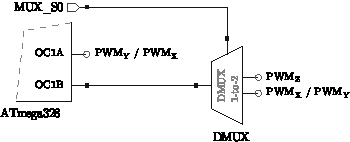
\includegraphics{drive_schem_pwm}
    \end{center}
Παρότι απεικονίζεται αντιστοίχιση του αποπολυπλέκτη με τον ακροδέκτη OC1B, θα
μπορούσε, κάλλιστα, να είχε γίνει με τον OC1A. Ο MUX\_S0 είναι ένας οποιοσδήποτε
ελεύθερος ακροδέκτης του μικροελεγκτή.
\end{figure}
